\documentclass{article}
\usepackage{amssymb}
\usepackage{amsmath}
\usepackage{centernot}
\usepackage{algpseudocode}
\usepackage{graphicx}
\usepackage[margin=1in]{geometry}
\setlength{\parindent}{0in}

\begin{document}

\title{EE360C: Lab 2}
\author{Joshua Dong (jid295)}
\date{\today}
\maketitle

\subsection*{Proof}
\subsection*{a) GPSR suboptimal}
Define a disjoint pair of paths is a pair of paths that share no nodes in
range of each other except for source and sink. Suppose the transmission range
is small relative to the distance between source and sink and we draw a circle
connecting both source and sink, placing stations on the circle in a sparse
way but constructiong two paths. These paths are disjoint since their only
nodes in range are source and sink.

Suppose there exists an arbitrary pair of disjoint paths of significantly
differing length where both paths are could be selected by the GPSR algorithm
had the other path not existed. Then take the more optimal path and change the
second node to a locally suboptimal node (connecting it to the rest of the
path). Then the path we modified is still more optimal, but will not be
selected by the GPSR algorithm. Then the GPSR algorithm is not optimal.

\subsection*{b) Dijkstra better than GPSR}
Dijkstra is proven to be correct. Since $dijkstraPathHops$ optimizes for path
hops, then it must do better or equal to GPSR for path hops. GPSR is not correct
so it does not do better than a correct solution.

$dijkstraPathHops$ does not provide an optimal solution to routing since path
hops do not take into account latency. For example, a connection in the path
returned by $dijkstraPathHops$ may have an unusually high latency, which would
lead to a suboptimal result in terms of minimum latency.


\subsection*{Efficiency}
\subsection*{a) Memory}
My graph representation has a memory efficiency of $O(n^2)$, where n is the
number of verticies. This is because we sore all the verticies mapped to every
edge in radius. The maximum number of edges is of order $n^2$.

There was an optimization in that we only stored verticies in range for the
map. We used a hash map to the edges to reduce look up time for hubs in range.

\subsection*{b) Runtime}
Space is not too important here relative to computation, since with our
optimization of only storing verticies in range, we are actually closer to
average $O(n)$ memory usage.

Our computation of the graph is $O(m + n)$, or simply $O(n)$ for n edges and m
verticies. This is because we need to loop through the verticies and edges,
but there are more edges than verticies, so the number of verticies is dominated
by the edges in a connected graph (our assumption for analysis).


\subsection*{c) Dijkstra Runtime}
Keeping the assumption of a connected graph (a few exceptions do not affect
our complexity), our complexity is $O(n^2)$ for n edges and m verticies. We
must iterate through all the relevant edges for every node we visit, a edge
for every node in range. In a fully connected graph this would mean a $n - 1$
edges to check for each node.

\subsection*{Runtime Efficiency and Success Rate}
\subsection*{a) gpsr}
\begin{verbatim}
---------------------------
Results for the input graph
---------------------------

Transmission Range = 5.0 meters.

The GPSR algorithm is successful 4950/4950 times.
The average time taken by the GPSR algorithm on successful runs is 9102 nanoseconds.

Transmission Range = 10.0 meters.

The GPSR algorithm is successful 4950/4950 times.
The average time taken by the GPSR algorithm on successful runs is 4217 nanoseconds.

Transmission Range = 15.0 meters.

The GPSR algorithm is successful 4950/4950 times.
The average time taken by the GPSR algorithm on successful runs is 876 nanoseconds.

Transmission Range = 20.0 meters.

The GPSR algorithm is successful 4950/4950 times.
The average time taken by the GPSR algorithm on successful runs is 880 nanoseconds.

Transmission Range = 25.0 meters.

The GPSR algorithm is successful 4950/4950 times.
The average time taken by the GPSR algorithm on successful runs is 893 nanoseconds.
\end{verbatim}

\subsection*{b) dijkstraAllPairsLatency}
\begin{verbatim}
---------------------------
Results for the input graph
---------------------------

Transmission Range = 5.0 meters.

Dijkstra's algorithm (Min Latency) is successful 4950/4950 times.
The average time taken by Dijkstra's algorithm (Min Latency) on successful runs is 319894 nanoseconds.

Transmission Range = 10.0 meters.

Dijkstra's algorithm (Min Latency) is successful 4950/4950 times.
The average time taken by Dijkstra's algorithm (Min Latency) on successful runs is 278334 nanoseconds.

Transmission Range = 15.0 meters.

Dijkstra's algorithm (Min Latency) is successful 4950/4950 times.
The average time taken by Dijkstra's algorithm (Min Latency) on successful runs is 277976 nanoseconds.

Transmission Range = 20.0 meters.

Dijkstra's algorithm (Min Latency) is successful 4950/4950 times.
The average time taken by Dijkstra's algorithm (Min Latency) on successful runs is 286133 nanoseconds.

Transmission Range = 25.0 meters.

Dijkstra's algorithm (Min Latency) is successful 4950/4950 times.
The average time taken by Dijkstra's algorithm (Min Latency) on successful runs is 276340 nanoseconds.
\end{verbatim}


\subsection*{c) dijkstraAllPairsHops}
\begin{verbatim}
---------------------------
Results for the input graph
---------------------------

Transmission Range = 5.0 meters.

Dijkstra's algorithm (Min Hops) is successful 4950/4950 times.
The average time taken by Dijkstra's algorithm (Min Hops) on successful runs is 366948 nanoseconds.

Transmission Range = 10.0 meters.

Dijkstra's algorithm (Min Hops) is successful 4950/4950 times.
The average time taken by Dijkstra's algorithm (Min Hops) on successful runs is 310125 nanoseconds.

Transmission Range = 15.0 meters.

Dijkstra's algorithm (Min Hops) is successful 4950/4950 times.
The average time taken by Dijkstra's algorithm (Min Hops) on successful runs is 321465 nanoseconds.

Transmission Range = 20.0 meters.

Dijkstra's algorithm (Min Hops) is successful 4950/4950 times.
The average time taken by Dijkstra's algorithm (Min Hops) on successful runs is 315379 nanoseconds.

Transmission Range = 25.0 meters.

Dijkstra's algorithm (Min Hops) is successful 4950/4950 times.
The average time taken by Dijkstra's algorithm (Min Hops) on successful runs is 325333 nanoseconds.
\end{verbatim}

\subsection*{d) Plot}
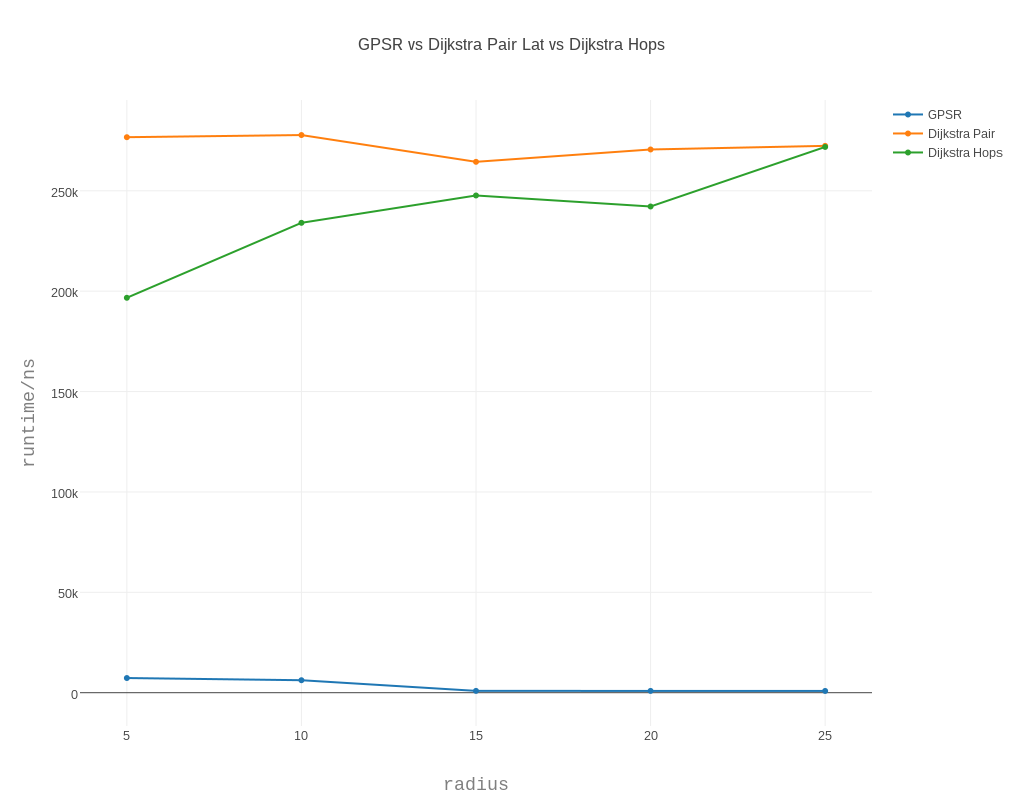
\includegraphics[width=\linewidth]{../graph/plot.png}

Greater vertex radius meant more searching, a bit slower for performance.
Depending on requirements of application, GPSR may be suitable because it is
quite fast relative to Dijkstra's algorithm. The two versions of Dijkstra's
algorithm are similar, but it appears that the dijkstra algorithm optimizing
for hops has a relatively small advantage time-wise against the
latency-optimal solution.

\end{document}
